\subsubsection{11.12.14}

\begin{enumerate}
	\item Время начала и окончания собрания: 17:30 - 23:30
	\item Цели собрания:
	\begin{enumerate}
		\item Установить стальные перекладины на подъемник.
		
		\item Добавить второй сервопривод на механизм опрокидывания ковша.
		
		\item Упаковать робота для транспортировки на соревнования "Робофест-Рязань".
	\end{enumerate}
	\item Проделанная работа:
	\begin{enumerate}
		\item Была установлена еще одна стальная перекладина. Всего их установлено две из трех. На перекладине, неподвижно закрепленной на роботе, решено было оставить прежнюю алюминиевую ось, на которую надета трубка, так как стальная ось из-за чуть большего диаметра (примерно на 0.1мм) не входила в трубку. Мы решили не стачивать стальную ось, поскольку алюминиевая ось почти не изгибалась благодаря надетой на нее трубке и, кроме того, трубка имела возможность проворачиваться на алюминиевой оси, что способствовало уменьшению силы трения.
		
		\item Для дополнительного уменьшения силы трения между осью и трубкой, они были хорошо нами смазаны.
		
		\begin{figure}[H]
			\begin{minipage}[h]{0.2\linewidth}
				\center  
			\end{minipage}
			\begin{minipage}[h]{0.6\linewidth}
				\center{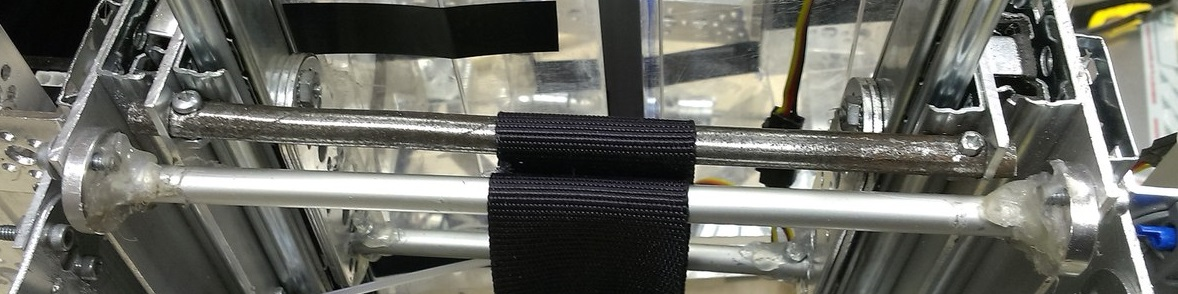
\includegraphics[scale=0.3]{days/10.12.14/images/01}}
				\caption{Неподвижная перекладина смазана}
			\end{minipage}
		\end{figure}
		
		\item Два сервопривода оказались также неспособны опрокинуть ковш, поэтому было решено переместить механизм опрокидывания ковша на прежнее место (в центральной части последней пары мебельных реек).
		
		\item Робот упакован для транспортировки.
		
	\end{enumerate}
	\item Итоги собрания:
	\begin{enumerate}
		\item Стальные перекладины установлены.
		
		\item Сервоприводы, опрокидывющие ковш было решено переместить на прежнее место.
		
		\item Сервоприводы не перенесены.
		
	\end{enumerate}
	\item Задачи для последующих собраний:
	\begin{enumerate}	
		\item Переместить на прежнее место сервоприводы, опрокидывающие ковш.
		
		\item Потренироваться в управлении роботом перед соревнованиями.
		
		\item Поставить на ковш механизм, который будет направлять шарики перпендикулярно земле.
		
	\end{enumerate}
\end{enumerate}
\fillpage